\chapter{Concept}

\section{Overview}
Johannes

\section{Hardware structure}
The hardware is design to allow an easy exchange of components and extensions. A FPGA is used as main computation unit. All components used by the car are connected to this central unit. The communication between the car's components uses ethernet. This is also used for car2x communication through a wiport. Every wheel is controlled by a single nano FPGA, which uses an UART-to-ethernet converter to communicate with the main FPGA. A schematic structure can be seen in figure \ref{HWconc}.
\begin{center}
\begin{figure}[h]
	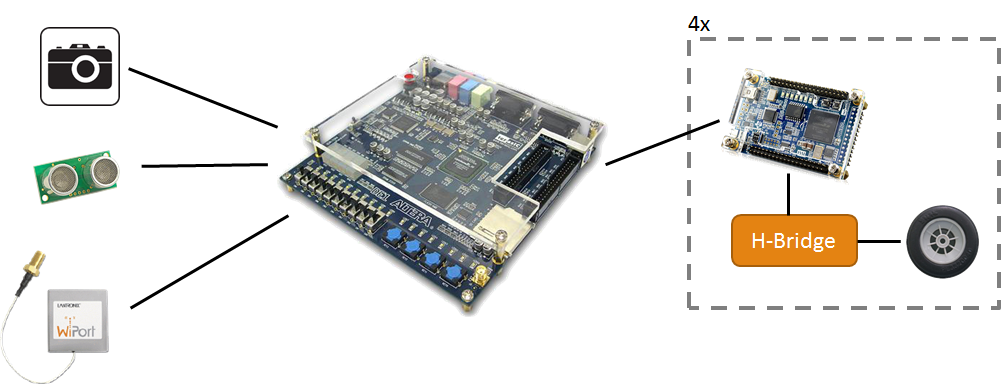
\includegraphics[width=\textwidth]{figures/hardwareconcept.png}
	\caption{Schematic hardware structure} \label{HWconc}
\end{figure}
\end{center}

\section{Communication Flow}
Paul - done

\section{Car2X Protocol}
The „CARP protocol"(developped by a previous lab-course group) was extended by a set of messages to let the NIOS2 processor system fit into the role of the communication central of the car. One NIOS2 core is handling the internal state of the car and the other one is in charge of all the communication between internal car parts and external communication partners like other cars or “car2x” stations. \newline
The internal communication protocol is based on the work of Florian Hisch and has nearly not been modified. The only major change was a role switch in terms of server-client relationship. Unlike before, the central unit now is a server to which external clients can connect to.
Keeping that in mind, there now is an external communication interface featuring the so called "Car2X-Messages" as an extension of the “CARP protocol”. Each message of this type, which is sent to the car, will be answered by the car after being processed or getting outdated. 
\newline
All this behaviour is handled on the "communication-core" of the NIOS2 system.
By parsing in the messages in the “socketserver.cpp” file directly from the incoming TCP/IP byte stream, there is a new message object created for every new message.
After that, the "sss exec command()" function handles the received message by reading out the message type an then taking various steps depending on the specific message.

